% Research-paper writeup for the single-SKU inventory-replenishment RL project.
% Overleaf- and pdflatex-ready: single file, only standard packages.
% Build locally:  pdflatex report.tex  (run twice for the table of contents / references)
% Figures are resolved from ../figures (repo build) or ./figures (if uploaded alongside on Overleaf).

\documentclass[11pt]{article}

\usepackage[margin=1in]{geometry}
\usepackage{graphicx}
\usepackage{booktabs}
\usepackage{amsmath,amssymb}
\usepackage{xcolor}
\usepackage[hidelinks]{hyperref}
\usepackage{caption}
\usepackage{enumitem}

% Resolves figures whether built from paper/ (repo), or on Overleaf with the PNGs in a
% figures/ subfolder or uploaded alongside this .tex at the project root.
\graphicspath{{../figures/}{figures/}{./}}
\captionsetup{font=small}
\setlist{nosep,leftmargin=1.4em}

\title{\textbf{Reinforcement Learning for Single-SKU Inventory Replenishment:\\
a Tabular Agent Benchmarked Against the Newsvendor Optimum}}
\author{Khai Lap Vuong\\[2pt]
\small Desautels Faculty of Management, McGill University\\
\small \emph{Designing \& Building Agentic AI Systems} (MMA)}
\date{}

\begin{document}
\maketitle

\begin{abstract}
\noindent
We frame periodic-review inventory replenishment for a single product as a finite-horizon
Markov Decision Process and study whether reinforcement learning (RL) adds value over the
classical newsvendor base-stock policy. Using a small, fully inspectable simulator, we train a
tabular Q-learning agent (with a Stable-Baselines3 PPO agent as a stretch) and evaluate it on
$100$ held-out demand episodes with a paired design, bootstrap confidence intervals, and a
Wilcoxon signed-rank test. The central finding is deliberately unglamorous and honest: under
stationary demand a correctly specified base-stock policy is near-optimal, and the learned agent
\emph{ties} it (within $3.3\%$) rather than beating it. RL earns its keep only under
non-stationarity: a season-aware agent matches a hand-built time-indexed base-stock and beats a
static one by roughly \$500 per episode, \emph{recovering the seasonal solution from reward
alone, without being given the seasonal model}. We then make the project's safety argument
empirical. Training the same agent on a tempting proxy objective (``minimize stockouts'')
improves the service-level dashboard while destroying $38.5\%$ of profit---the textbook
reward-hacking failure---and a worst-case policy floods the warehouse to $20\times$ capacity
unless a hard constraint, enforced in code rather than reward, bounds it. All four failure modes
named by the brief (reward hacking, instability, overfitting, unsafe behavior) are
\emph{measured}, not asserted, and the deployment recommendation (shadow first) follows directly
from that evidence.
\end{abstract}

\tableofcontents
\medskip
\hrule

\section{Introduction and problem framing}
\label{sec:intro}

Inventory replenishment is a repeated decision under uncertainty: each period a planner observes
stock and chooses how much to reorder, an order arrives after a lead time, demand is random, and
unmet demand is lost. The decision is genuinely \emph{sequential}---an order placed today arrives
later and the stock it brings becomes a holding cost or a stockout tomorrow---so it cannot be
reduced to a one-shot (bandit) choice. That delayed-consequence structure is exactly what
RL is designed for, and it is the reason this problem sits above the contextual-bandit rung of
the modelling ladder.

The interesting question is not ``can an agent learn to order stock?'' but ``does learning add
value over the operations-research answer we already have, and what could go wrong if we deploy
it?'' We answer both honestly. Our contributions are:
\begin{itemize}
  \item A clean MDP formulation of single-SKU replenishment with an analytically derived
        newsvendor benchmark (Section~\ref{sec:mdp}).
  \item An explicit \emph{balanced} reward and a deliberately gameable \emph{naive} reward that
        turn the reward-hacking lesson into a measured experiment (Section~\ref{sec:reward}).
  \item A paired, held-out evaluation showing the agent ties the optimum under stationary demand
        and adapts under seasonality (Sections~\ref{sec:eval}--\ref{sec:results}).
  \item Quantified failure analysis across all four named failure modes, plus a hyperparameter
        and seed robustness study (Section~\ref{sec:failure}).
  \item A deployment recommendation argued from the evidence (Section~\ref{sec:deploy}).
\end{itemize}

\section{The world as a Markov Decision Process}
\label{sec:mdp}

We model one SKU under periodic review with lead time $L$ and lost sales. The MDP
$(\mathcal{S},\mathcal{A},P,R,\gamma)$ over a finite horizon $H$ is:

\begin{description}
  \item[State $\mathcal{S}$.] The \emph{inventory position} $\mathrm{IP}=\text{on-hand}+\text{pipeline}$
        (stock plus in-transit orders)---the sufficient statistic for ordering. A coarse season
        \emph{phase} is appended for the seasonal agent (Section~\ref{sec:markov}).
  \item[Action $\mathcal{A}$.] An order quantity from the discrete menu
        $\{0,5,10,15,20,25,30\}$.
  \item[Transition $P$.] Receive the order placed $L$ periods ago; place a (clamped) order;
        realize $\mathrm{Poisson}$ demand; sell what stock allows and lose the rest.
  \item[Reward $R$.] The per-period profit of Eq.~\eqref{eq:reward}.
  \item[Discount $\gamma=0.99$.] A mild time preference over the finite horizon.
  \item[Horizon $H=52$ weeks] (one season).
\end{description}

\paragraph{Economics and the newsvendor benchmark.}
Price $p=10$, unit cost $c=4$ (margin $6$), holding cost $h=1$ per unit per period, and
stockout penalty $b=5$ per unit. The single most important modelling fact is the
\emph{underage} cost. Under lost sales, being one unit short forfeits the margin that unit would
have earned \emph{and} the goodwill penalty:
\begin{equation}
  C_u = (p-c) + b = 11, \qquad C_o = h = 1, \qquad
  \mathrm{CR} = \frac{C_u}{C_u + C_o} = \frac{11}{12} \approx 0.917 .
\end{equation}
Counting only the penalty ($C_u=b=5$) is the classic newsvendor error; it would understate the
order-up-to level and weaken the very baseline we must beat. For periodic review with lead time
$L=1$ the protection interval is $L+1=2$ periods, so the order-up-to level is the critical
quantile of two-period demand,
\begin{equation}
  S = \big\lceil F^{-1}_{\mathrm{Poisson}(2\lambda)}(\mathrm{CR}) \big\rceil
    = \big\lceil F^{-1}_{\mathrm{Poisson}(20)}(0.917) \big\rceil = 26 .
\end{equation}

\paragraph{Hard constraints are part of the world, not the reward.}
Two limits are enforced by the environment \emph{before} an order is placed: a per-order cap
($0\le \text{order}\le 30$) and a warehouse-capacity cap ($\text{on-hand}\le 50$). Orders above a
review threshold ($25$ units) are flagged for human approval. These are physical/policy
constraints the agent must never cross; encoding them as code rather than as reward penalties is
what makes the safety guarantee hold regardless of what the agent learns
(Section~\ref{sec:failure}).

\paragraph{The Markov property and partial observability.}
\label{sec:markov}
Under stationary demand the problem is Markov in $\mathrm{IP}$, so a state of $\mathrm{IP}$ bins
suffices. Under \emph{seasonal} demand it is not: the demand rate depends on the week, so
$\mathrm{IP}$ alone is partially observable and the agent needs a time feature. This is not a
footnote---it is measured. The $\mathrm{IP}$-only agent scores $2253$ under seasonality while the
phase-augmented agent scores $2588$ (Table~\ref{tab:results}); the $335$-point gap is a
\emph{partial-observability} failure, not an algorithm failure.

\section{Reward design}
\label{sec:reward}

The reward is where business strategy becomes a number, and it is the project's central
experiment. We use cost-at-order accounting:
\begin{equation}
  R_t = p\cdot \text{sales}_t - c\cdot \text{order}_t - h\cdot \text{on-hand}_{t+1}
        - b\cdot \text{unmet}_t - K\cdot \mathbb{1}[\text{order}_t>0]
        \;(+\, s_v\cdot \text{on-hand}_H \text{ at the horizon}).
  \label{eq:reward}
\end{equation}
Paying for orders at placement (rather than netting margin on sales) makes the terminal salvage
$s_v$ coherent---leftover stock is cash already spent, partially recovered---and removes an
end-of-horizon sell-down artifact. The per-period ordering trade-off is still governed by
$C_u$ and $C_o$, so $S=26$ is unchanged.

Against this we define a deliberately \emph{gameable} proxy that rewards only service:
$R^{\text{naive}}_t = -\,b\cdot \text{unmet}_t$. Optimizing it satisfies the service KPI by
ordering to the warehouse cap. Training an agent on the proxy and then \emph{scoring} it on the
true objective (Eq.~\eqref{eq:reward}) makes the reward-hacking lesson empirical rather than
rhetorical (Section~\ref{sec:failure}).

\section{Methods and system architecture}
\label{sec:methods}

\paragraph{Baselines (the ladder).}
We climb the modelling ladder only as far as the problem demands and benchmark RL against the
strongest simple policy: (i) \texttt{random} (the floor); (ii) \texttt{base\_stock}, order-up-to
$S=26$ from the newsvendor quantile (the near-optimal stationary anchor); (iii)
\texttt{seasonal\_base\_stock}, a week-indexed $S_t$ (the fair adaptive competitor under
seasonality); and (iv) an $(s,S)$ variant for the fixed-order-cost case. To compete on the same
footing, each baseline's continuous order is snapped to the discrete action menu.

\paragraph{Tabular Q-learning (primary).}
The state space is small once we act on inventory position, so a table is the right tool: it
converges in seconds, every value is inspectable, and the greedy policy can be plotted against
base-stock. The update is the standard
\begin{equation}
  Q(s,a) \leftarrow Q(s,a) + \alpha\big[r + \gamma \max_{a'} Q(s',a') - Q(s,a)\big],
\end{equation}
with a Robbins--Monro learning rate $\alpha = 1/(1+\text{visits}(s,a))$, $\gamma=0.99$,
$\varepsilon$ annealed $1.0\!\to\!0.05$, over $30{,}000$ episodes. Inventory position is binned
in steps of $5$ ($11$ bins); a $13$-bucket season phase is added for the seasonal agent.

\paragraph{PPO (stretch).}
A Stable-Baselines3 PPO agent trains on a Gymnasium wrapper of the same environment. It is the
stretch, not the headline: on this small problem it is slower, seed-variable, and lands
\emph{below} the tabular agent (Section~\ref{sec:results}), which is itself the clearest argument
for the baseline ladder.

\paragraph{Architecture.}
The codebase is a small acyclic layering: \texttt{config} (frozen parameter dataclasses)
$\rightarrow$ \texttt{rewards}, \texttt{demand} $\rightarrow$ \texttt{env} (the Gymnasium
simulator with the hard clamps) $\rightarrow$ policies (\texttt{baselines}, \texttt{q\_learning},
\texttt{ppo\_agent}) $\rightarrow$ \texttt{evaluation} (pure measurement) $\rightarrow$
\texttt{experiments} (orchestration) $\rightarrow$ \texttt{plotting}, \texttt{cli}. The reward
carries the objective; the environment carries the safety limits; the agents only choose actions.

\section{Evaluation methodology}
\label{sec:eval}

Rigour, not model size, is where the result lives. Every policy is scored on $100$ \emph{held-out}
demand episodes drawn from a seed stream disjoint from training (separation asserted in code, so
``out-of-sample'' is proven, not assumed). The design is \emph{paired}: every policy faces the
identical demand realization per episode, so differences reflect the policy, not luck. We report
the mean return with a $95\%$ \emph{paired-bootstrap} confidence interval, a Wilcoxon
signed-rank test as the primary significance check (paired $t$ as a cross-check), and the dollar
effect size rather than a bare $p$-value. Because risk-averse operations care about bad weeks, we
also report the $5$th-percentile (\texttt{p05}) downside-tail return. Returns are always computed
under the balanced reward, even for the proxy-trained agent: you optimize the proxy, but you are
graded on the business. To make the comparison fair, base-stock is evaluated on the same discrete
action menu as the agent, and no hyperparameter is tuned on the held-out set.

\section{Results}
\label{sec:results}

\begin{table}[t]
\centering
\caption{Held-out performance over $100$ paired episodes (one 52-week season each). Mean return
in \$ with $95\%$ paired-bootstrap CI; \texttt{p05} is the 5th-percentile downside return. The
near-optimal baseline per regime is in \textbf{bold}.}
\label{tab:results}
\begin{tabular}{llrr}
\toprule
Regime & Policy & Mean return [95\% CI] & p05 \\
\midrule
stationary  & \textbf{base\_stock} ($S{=}26$) & \textbf{2673.9} [2648, 2699] & 2425 \\
            & q\_learning (tabular)        & 2585.6 [2558, 2613] & 2338 \\
            & ppo (stretch)               & 2538.7 [2513, 2563] & 2316 \\
            & random                      & 1792.6 [1757, 1828] & 1506 \\
\midrule
seasonal    & \textbf{seasonal\_base\_stock} ($S_t$) & \textbf{2666.8} [2636, 2699] & 2434 \\
            & q\_learning (phase-aware)   & 2588.0 [2557, 2621] & 2348 \\
            & q\_learning (IP-only)       & 2252.6 [2226, 2280] & 2043 \\
            & static\_base\_stock ($S{=}26$) & 2086.7 [2063, 2110] & 1885 \\
            & ppo (stretch)               & 1928.9 [1894, 1965] & 1632 \\
            & random                      & 1426.6 [1371, 1482] & \phantom{0}966 \\
\bottomrule
\end{tabular}
\end{table}

\paragraph{Does RL beat the baseline? Honestly, no---and it should not.}
Under stationary demand the correctly specified base-stock policy is near-optimal, and tabular
Q-learning lands within $3.3\%$ of it: a mean gap of $-\$88$ per episode ($95\%$ CI
$[-98,-79]$, Wilcoxon $p\approx 3\times10^{-17}$). This is the point---a \emph{negative} result
that shows RL is not being oversold on a problem operations research already solves
(Figure~\ref{fig:comparison}).

\paragraph{When RL earns its keep.}
Under seasonal demand a \emph{static} base-stock is misspecified and loses $-\$580$ per episode
relative to a time-indexed $S_t$. The phase-aware agent recovers nearly all of that, tying the
seasonal base-stock (gap $-\$79$, CI $[-91,-66]$) and beating the static rule by $\approx\$500$
per episode. Crucially, it does so \emph{without being handed the seasonal model}: it learns the
time-varying order-up-to target from reward alone (Figure~\ref{fig:behavior}, right). The honest
caveat: a planner who can write the seasonal rule down does not need RL; RL hedges against
\emph{not} knowing it.

\begin{figure}[t]
\centering
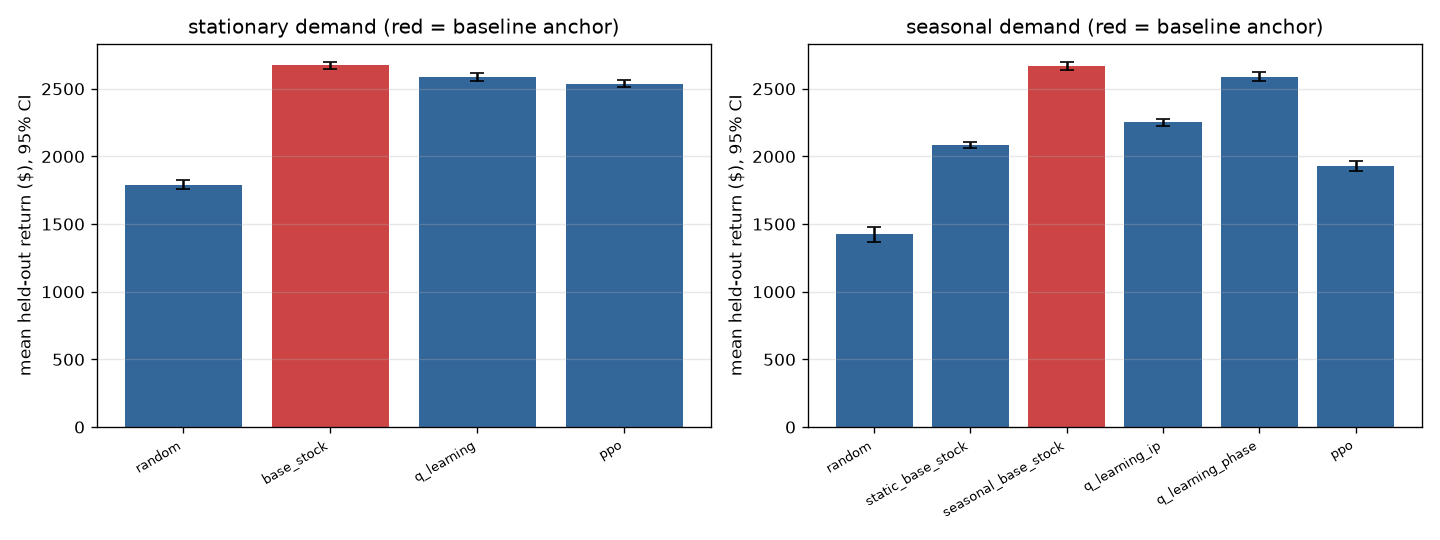
\includegraphics[width=0.85\linewidth]{policy_comparison.png}
\caption{Mean held-out return with $95\%$ CIs, by policy and regime. Left: stationary (the agent
ties the base-stock anchor). Right: seasonal (the phase-aware agent ties the seasonal base-stock
and beats the misspecified static one).}
\label{fig:comparison}
\end{figure}

\begin{figure}[t]
\centering
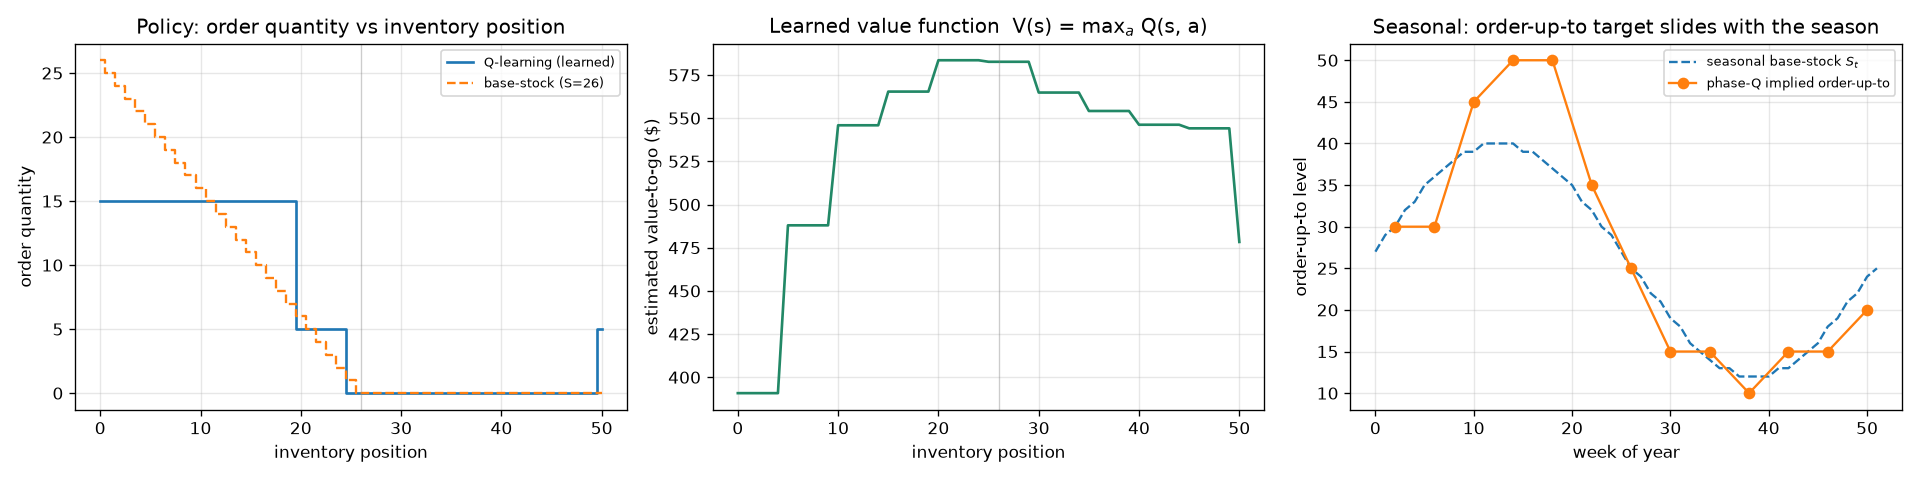
\includegraphics[width=0.97\linewidth]{policy_behavior.png}
\caption{Left: the learned order curve traces the base-stock staircase (order hard when empty,
stop near $S=26$). Middle: the learned value function $V(s)=\max_a Q(s,a)$ peaks at moderate
inventory and falls off toward stockout and overstock---the shape the Bellman recursion predicts.
Right: the phase agent's implied order-up-to level slides with the season, tracking $S_t$.}
\label{fig:behavior}
\end{figure}

\paragraph{Convergence and stability.}
Tabular returns climb smoothly and settle well within budget. PPO, shown across seeds in
Figure~\ref{fig:reward_curve}, is both slower to converge and visibly seed-variable, and lands
below the tabular agent---deep RL buys variance, not value, on a problem this small.

\begin{figure}[t]
\centering
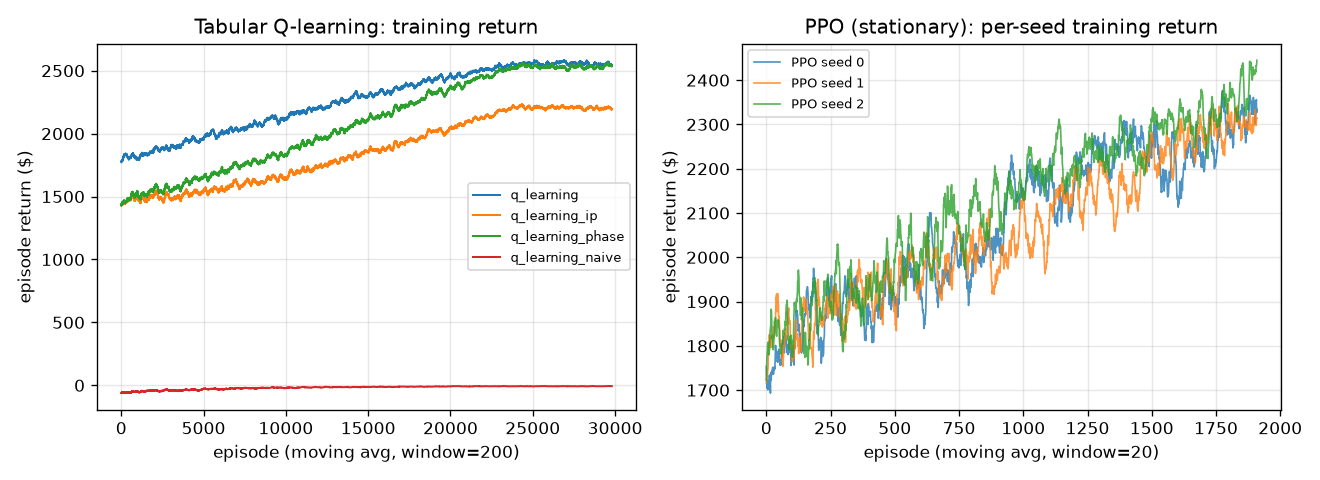
\includegraphics[width=0.97\linewidth]{reward_curve.png}
\caption{Training-return curves. Left: tabular Q-learning (smooth convergence). Right: PPO across
three seeds (visible spread; sample-inefficient relative to the table).}
\label{fig:reward_curve}
\end{figure}

\section{Failure analysis}
\label{sec:failure}

We measure each of the four named failure modes rather than asserting them
(Table~\ref{tab:failure}).

\paragraph{Reward hacking (the headline safety result).}
Trained on the service-only proxy, the agent games it perfectly: service rises to $0.997$ (from
$0.989$) while true economic return \emph{falls} $38.5\%$ ($-\$995$ per episode), as it floods
the warehouse to $29$ units on-hand (vs.\ $9$) and holding cost explodes
(Figure~\ref{fig:reward_hacking}). The proxy was satisfied; the business was not---and the
service dashboard would not have warned us. The capacity cap bounded the damage, but capacity is
the only thing that did.

\paragraph{Unsafe behavior (safety ablation).}
To show the guarantee comes from the environment rather than the policy, we run a worst-case
always-max-order policy with the capacity clamp on versus off. With the clamp \emph{off}, on-hand
peaks at $1{,}023$ units ($49$ violations); with it \emph{on}, on-hand never exceeds $39$ ($0$
violations). Safety is enforced in code, not learned.

\paragraph{Overfitting / generalization.}
Under a permanent demand shift ($\lambda\!:\!10\!\to\!16$), we score both the $\lambda=10$-tuned
agent and base-stock against an \emph{oracle} base-stock recomputed for $\lambda=16$. The result
\emph{corrected our prior}: the learned policy tracks the oracle more closely (gap-to-oracle
$685$) than the statically tuned $S=26$ rule (gap $1{,}549$), because the fixed rule rigidly
under-stocks once demand rises. (Caveat: this is one shift direction; either policy should be
re-fit when the regime changes.)

\paragraph{Instability and robustness.}
PPO's three training seeds finish at $2303/2299/2369$---a real spread that disqualifies any
single-seed claim. The tabular result, by contrast, is robust: across bin widths $2$--$10$ the
gap to base-stock holds at $-83/-88/-87$, collapsing only when bins are too coarse to represent
the order-up-to structure (width $25$, $3$ states, $-5125$); across three training seeds the
held-out return varies by only $\$35$ ($2586/2612/2621$). We also confirmed the finite-horizon
tail is not a confound: the stationary agent's state omits the week, so it cannot exploit the
horizon, and its last-period waste ($\$41.6$) is within $\$2.4$ of base-stock's ($\$39.2$).

\begin{table}[t]
\centering
\caption{The four failure modes, each measured. ``True return'' is always under the balanced
objective.}
\label{tab:failure}
\begin{tabular}{lll}
\toprule
Failure mode & Probe & Result \\
\midrule
Reward hacking & train on ``minimize stockouts'' & service $0.997$ vs $0.989$; profit $-38.5\%$; on-hand $29$ vs $9$ \\
Unsafe behavior & remove the capacity clamp & peak on-hand $1023$ ($49$ viol.) vs $39$ ($0$ viol.) \\
Overfitting & shift $\lambda\,10\!\to\!16$ vs oracle & gap-to-oracle $685$ (Q) vs $1549$ (static base-stock) \\
Instability & PPO across $3$ seeds & final returns $2303/2299/2369$ (vs deterministic tabular) \\
\bottomrule
\end{tabular}
\end{table}

\begin{figure}[t]
\centering
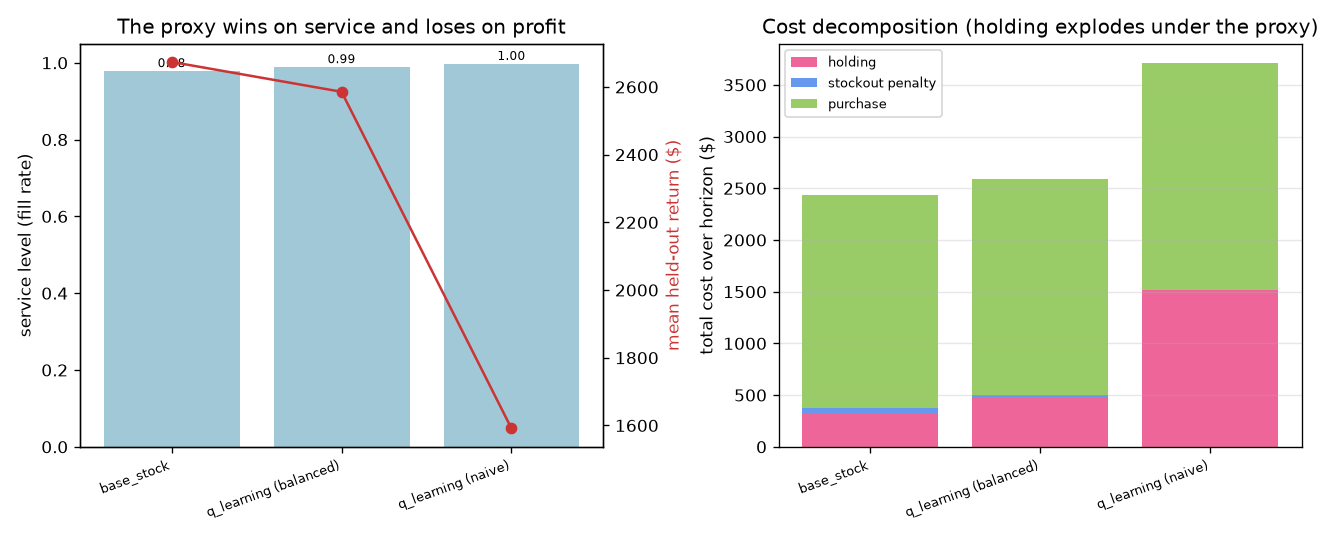
\includegraphics[width=0.97\linewidth]{reward_hacking.png}
\caption{Reward hacking. Left: the proxy agent wins on service (bars) and loses on economic
return (line). Right: cost decomposition---holding cost explodes under the proxy while the
balanced agent stays near the base-stock profile.}
\label{fig:reward_hacking}
\end{figure}

\section{Deployment discussion}
\label{sec:deploy}

The recommendation follows from the evidence: \textbf{shadow first, do not yet automate}. The
agent only ties the incumbent under stable demand, and the reward-hacking result shows that the
cost of any objective mis-specification is severe and KPI-invisible. Yet the seasonal adaptivity
is real and the safety limits hold, so rejecting the agent would forfeit genuine value. We
therefore propose a guarded rollout in which friction scales with consequence: (1) shadow mode
(agent recommends, buyers execute the incumbent; compare realized profit/service); (2)
human-in-the-loop (agent default, buyer approves large orders); (3) limited autonomy on low-risk
SKUs with an automatic rollback if weekly profit drops below the incumbent's trailing average or
any capacity flag fires; (4) broad autonomy only after a full season of evidence. Rollback is
cheap by construction---the incumbent base-stock policy is a one-line formula, and every agent
decision writes a full trace. The agent pays for itself precisely on the SKUs whose demand we
\emph{cannot} model well, not the easy stationary ones.

\section{Limitations and reflection}
\label{sec:limitations}

This is a scoped teaching artifact, and we state its limits plainly. (i) It is one SKU with
synthetic Poisson demand and a fixed lead time; real demand is correlated, censored, and
promotion-driven. (ii) Under lost sales, base-stock is a strong heuristic, not the proven
optimum, so a tiny RL edge is theoretically possible; our CIs show the stationary gap is small
and \emph{against} RL, so we report the honest tie. (iii) The discretization has a safe range,
not infinite headroom (it collapses at $\ge 25$-unit bins). (iv) The balanced reward is itself
\emph{a model} of the objective---better than the naive one, but the whole project is a warning
about shipping a confident agent built on a wrong reward.

The build also corrected several of our own priors, which we view as the signature of real
engineering rather than a weakness: we nearly mis-specified the underage cost ($C_u=b$ instead of
$(p{-}c){+}b$); the seasonal ``win'' was dishonest until we added the seasonal base-stock as the
fair competitor; and the overfitting probe contradicted our assumption that the analytical rule
would generalize better. Each was resolved by measurement.

\section{Reproducibility}
\label{sec:repro}

Every source of randomness is a seeded \texttt{numpy} generator; there are no unseeded global
calls. Training, validation, and held-out evaluation use disjoint seed streams. The entire
tabular pipeline runs on CPU in $\sim$$135$ seconds with no GPU and no API keys, and a
from-scratch virtual environment built from the pinned lock reproduces the headline number
exactly (stationary Q-learning $=2585.6$). Each run stamps a deterministic \texttt{run\_id}
(a hash of seed, simulator fingerprint, and episode counts) into the committed report for
traceability.

\section{Conclusion}
\label{sec:conclusion}

On a problem operations research already solves well, the most useful thing an RL study can do is
tell the truth: the learned agent \emph{ties} the newsvendor optimum under stationary demand and
\emph{earns its keep only} by autonomously adapting to seasonality. The lasting value of the work
is the harness around the agent---the right baseline, paired held-out evaluation, hard safety
constraints, and a reward-hacking experiment that shows, in dollars, why the objective and the
constraints must be designed with as much care as the algorithm.

\begin{thebibliography}{9}
\bibitem{suttonbarto} R.~S. Sutton and A.~G. Barto. \emph{Reinforcement Learning: An
  Introduction}, 2nd ed. MIT Press, 2018.
\bibitem{mnih} V.~Mnih et al. Human-level control through deep reinforcement learning.
  \emph{Nature}, 518:529--533, 2015.
\bibitem{ppo} J.~Schulman, F.~Wolski, P.~Dhariwal, A.~Radford, and O.~Klimov. Proximal Policy
  Optimization Algorithms. \emph{arXiv:1707.06347}, 2017.
\bibitem{zipkin} P.~H. Zipkin. \emph{Foundations of Inventory Management}. McGraw-Hill, 2000.
\bibitem{zhengfedergruen} Y.-S. Zheng and A.~Federgruen. Finding optimal $(s,S)$ policies is about
  as simple as evaluating a single policy. \emph{Operations Research}, 39(4):654--665, 1991.
\bibitem{sb3} A.~Raffin et al. Stable-Baselines3: Reliable Reinforcement Learning
  Implementations. \emph{Journal of Machine Learning Research}, 22(268):1--8, 2021.
\bibitem{gymnasium} M.~Towers et al. Gymnasium: A Standard Interface for Reinforcement Learning
  Environments. \emph{arXiv:2407.17032}, 2024.
\end{thebibliography}

\end{document}
